\documentclass{anstrans}
%%%%%%%%%%%%%%%%%%%%%%%%%%%%%%%%%%%
\title{Adaptive Dynamic Event Tree in RAVEN code}
\author{Andrea Alfonsi, Cristian Rabiti, Diego Mandelli, Joshua Cogliati, Robert Kinoshita}

\institute{Idaho National Laboratory, 2525 Fremont Avenue, Idaho Falls, ID 83402, United States}

\email{$[andrea.alfonsi,cristian.rabiti,diego.mandelli,joshua.cogliati,robert.kinoshita]$@inl.gov}

% Optional disclaimer: remove this command to hide
%\disclaimer{Notice: This manuscript is a work of fiction. Any resemblance to actual articles, living or dead, is purely coincidental.}

%%%% packages and definitions (optional)
\usepackage{graphicx} % allows inclusion of graphics
\usepackage{booktabs} % nice rules (thick lines) for tables
\usepackage{microtype} % improves typography for PDF

\renewcommand{\vec}[1]{\bm{#1}} %vector is bold italic
\newcommand{\vd}{\bm{\cdot}} % slightly bold vector dot
\newcommand{\grad}{\vec{\nabla}} % gradient
\newcommand{\ud}{\mathop{}\!\mathrm{d}} % upright derivative symbol

\begin{document}
%%%%%%%%%%%%%%%%%%%%%%%%%%%%%%%%%%%%%%%%%%%%%%%%%%%%%%%%%%%%%%%%%%%%%%%%%%%%%%%%
\section{Introduction}

RAVEN ~\cite{ravenFY12,alfonsiMC,alfonsiESREL2014} is a software tool that is focused on performing statistical analysis of stochastic dynamic systems. RAVEN has been designed in a high modular and pluggable way in order to enable easy integration of different programming languages (i.e., C++, Python) and coupling with other applications (system codes). Among the several capabilities currently present in RAVEN, there are five different sampling strategies: Monte Carlo, Latin Hyper Cube, Grid, Adaptive and Dynamic Event Tree (DET) sampling methodologies~\cite{ravenFY14}. \\ The scope of this paper is to present a new sampling approach, currently under definition and implementation: an evolution of the DET method enhanced by the  sampling adaptivity features~\cite{mandelliSVMANS}. 


%%%%%%%%%%%%%%%%%%%%%%%%%%%%%%%%%%%%%%%%%%%%%%%%%%%%%%%%%%%%%%%%%%%%%%%%%%%%%%%%
\section{Dynamic Event Tree Methodology}
%Before analyzing the new adaptive approach, a short overview regarding the basic DET method needs to be reported. 
The DET technique brings several advantages~\cite{alfonsiPSA2013,ADAPTHakobyan} with respect the conventional event trees approach, among which the fact that it actually employs system simulators in order to model the actual accident evolution. In DET,  event sequences run simultaneously starting from a single initiating event. The branchings occur at user specified times and/or when an action is required by the operator and/or the system, creating a deterministic sequence of events based on the time of their occurrence (see Fig.~\ref{fig:detScheme}). 

This leads to a more realistic and mechanistically consistent analysis of the system taken in consideration. Thus, the DET methodology (along with other dynamic PRA methods) is designed to take explicitly into account the timing of events which can become very important especially when uncertainties in complex phenomena are considered. 

Starting from an initiating event, the main idea behind the DET methodology is to let a system code (i.e., RELAP5-3D, RELAP-7, etc.) determine the pathway of an accident scenario within a probabilistic ``environment''. \\ Figure~\ref{fig:detScheme} schematically shows the DET logic. Based on an user defined branching logic, driven by Probabilistic Density Functions (PDFs), an event occurs at a certain time instant. The simulation spoons $n$ different branches. In each of them, the branching event determines a different consequence (including an associated probabilities). Each sequence continues until another event occurs and a new set of branching is spooned. The simulation ends when an exit condition or a maximum mission time is reached.       
\begin{figure} % replace 't' with 'b' to force it to be on the bottom
  \centering
  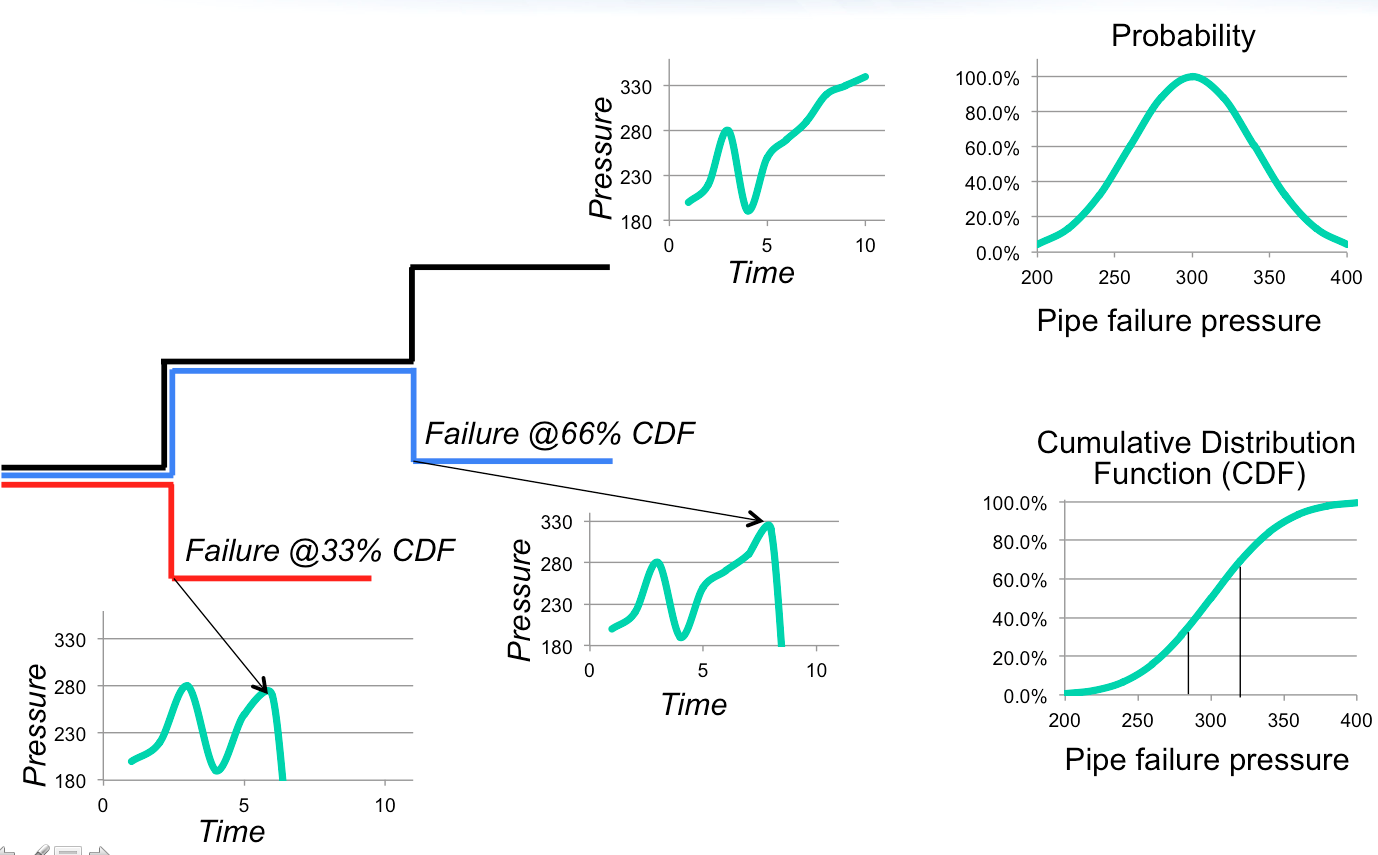
\includegraphics[width=0.4\textwidth]{detScheme.png}
  \caption{Dynamic Event Tree conceptual scheme}
  \label{fig:detScheme}
\end{figure} 
%%%%%%%%%%%%%%%%%%%%%%%%%%%%%%%%%%%%%%%%%%%%%%%%%%%%%%%%%%%%%%%%%%%%%%%%%%%%%%%%
\section{Adaptive Sampling}
The  adaptive methodology can be considered as a goal oriented sampling strategies for the research of limit surfaces (LSs). The LS is a hyper-surface, in the input space of the stochastic parameters, along which a specific goal function assumes an imposed value. 
%From a safety point of view, the limit surface  could be conveniently defined as the surface where $\begin{vmatrix} \overline{\triangledown} C\left ( \overline{x} \right ) \end{vmatrix} = \infty $, which simply is hyper surface that separates failure to success regions and where $C\left ( \overline{x} \right )$ is the goal function that defines the system behavior with respect the input space $\overline{x}$. 
%The information content of the LS image is rather minimal because it only illustrates a property of the goal function with respect the status of the system. 
It could be already noticed that the integration domain of the risk integral is the volume within the limit surface image $\partial V_{L}$:
\begin{equation} 
R=\int_{S\bigcap D} f _{\overline{X}}(\overline{x},t_{end})d\overline{x} =\int_{V_{L}}    f _{\overline{X}}(\overline{x},t_{end})d\overline{x}
\end{equation}
where, $D$ is the damaged space and the image of the limit surface $\partial V_{L}$ satisfies $\begin{vmatrix} \overline{\triangledown} C\left ( \partial V_{L} \right ) \end{vmatrix} = \infty $.
In most of the cases\cite{MathFrameworkMC2013}, the probabilistic behavior can be studied as a function of uncertainty in the model parameters and initial conditions.
Under this assumption, the phase space coordinates of the system at any moment in time is a function of $\overline{x}_{0}$, which represents the initial conditions and stochastic parameters characterizing the system. Therefore the system behavior can be now described by $\overline{x}(t)=h(\overline{x}_{0},t)$, where $h(\overline{x}_{0})$ is the mathematical model representing the system, once the initial conditions and the uncertain parameters are chosen. The probability propagates according:
\begin{equation} 
f _{\overline{X}}(\overline{x})d\overline{x} = f _{\overline{X}_{0}}(\overline{x}_{0})d\overline{x}_{0}
\end{equation}
As a consequence the risk integral can be evaluated as:
\begin{equation} 
R=\int_{h^{-1}(V_{L})} f _{\overline{X}_{0}}(\overline{x}_{0})d\overline{x}_{0}
\end{equation}
where $h^{-1}(V_{L})$ is the pre-image of $V_{L}$ and therefore $h^{-1}(\partial V_{L})$ is the limit surface.
\\
The knowledge of the LS allows a fast evaluation of risk functions, informs regarding which uncertainties are the most relevant from a risk point of view, defines safe areas to be explored for risk reduction, etc. Unfortunately, the search of a LS in terms of computational effort is very expensive, since a brute force approach would concern the evaluation of each point of a N-dimensional grid (with respect the input space),whose discretization is proportional to the wanted accuracy.
To avoid such a situation, RAVEN uses acceleration schemes based on surrogate models (SM), used to predict the location of the LS in order to guide the exploration of the input space close to relevant zones. 

\begin{figure} 
  \centering
     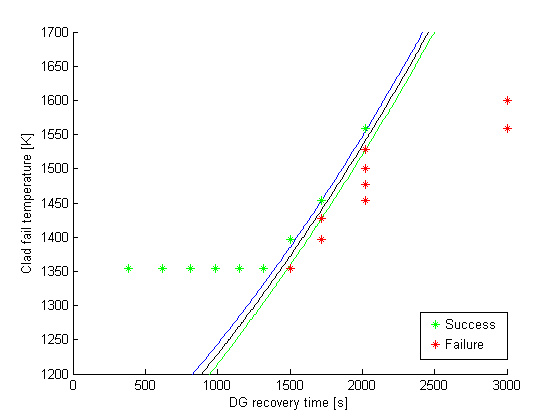
\includegraphics[width=0.5\textwidth]{DET_LS_pb.png}
  \caption{Dynamic Event Tree Limit Surface}
  \label{fig:LSDET}
\end{figure}

%%%%%%%%%%%%%%%%%%%%%%%%%%%%%%%%%%%%%%%%%%%%%%%%%%%%%%%%%%%%%%%%%%%%%%%%%%%%%%%%
\section{Dynamic Event Tree Adaptive sampling}
The main idea of the application of the previously explained sampling adaptivity to the DET approach comes from the observation that the DET, when evaluated from a LS perspective, is intrinsically adaptive.
\\ As an example, Figure~\ref{fig:LSDET}  shows a LS generated by the DET sampling methodology currently available in RAVEN. In this case, a goal function, based on the clad max temperature, is used; the DET method tends to search for the LS with a resolution equal to the user defined grid discretization, in the input space.
\begin{figure}
  \centering
     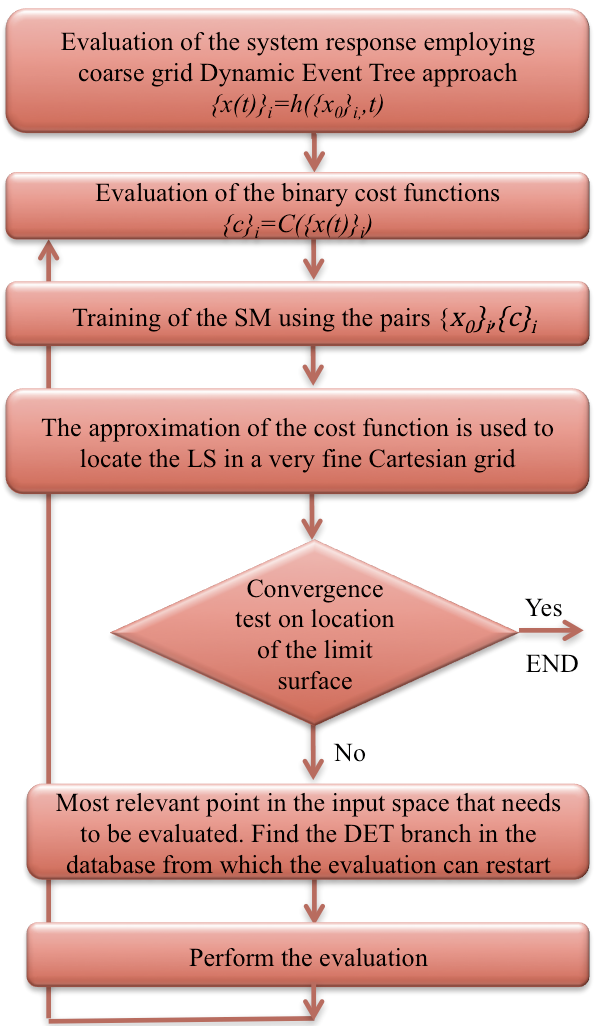
\includegraphics[width=0.35\textwidth]{AdaptiveDET.png}
  \caption{Adaptive Dynamic Event Tree Scheme}
  \label{fig:AdaptiveDET}
\end{figure}

For this reason, it appears natural to use the DET approach to perform a goal function oriented pre-sampling of the input space. The proposed approach can be described through the following steps (see Fig.~\ref{fig:AdaptiveDET}):
\begin{enumerate} 
\item A limited number of points in the input space $\overline{x}_{0i}$ are selected via a DET approach
\item The system code is used to compute the status of the system for the set of points in the input set:
\begin{equation}
    \overline{x}(t)=h(\overline{x}_{0i},t)
\end{equation}
\item The goal function (Boolean) is evaluated at the phase space coordinate of the system: 
\begin{equation}
g_{i}=G([\overline{x}(t)]_{i})
\end{equation}
\item The set of pairs $(\overline{x}_{0i},g_{i})$ are used to train a SM
\item The SM is used to predict the value of the goal function on a regular Cartesian grid in the domain space:
\begin{equation}
SM\left ( \left \{ \overline{x}_{0} \right \}_{j} \right ) \approx \left \{ c \right \}_{j}
\end{equation}
where $j=1, ..., M$ points on the grid 
\item The values of the goal function are used to determine the LS location based on the change of values of $\left \{ c \right \}_{j}$:
\begin{equation}
\left \{ c \right \}_{j} \rightarrow \partial V_{L}
\end{equation}
\item The position of the LS is compared with the one at the previous iteration; if no changes are detected, the iterations stop; otherwise a new point needs to be identified in the input space
\item The point located on the limit surface that is the farther from all the other already selected points is added to the $\overline{x}_{0i}$ set 
\item An hierarchical searching process is performed on the DET branches already evaluated and the starting point for the new evaluation is set
\item The process restart from point 2
\end{enumerate}

The DET approach, in conjunction with a LS search, is indicated for performing adaptive sampling, since, as already mentioned, the methodology itself can be considered a LS searching method. In this way, the adaptive sampling approach begins having a SM trained with a solution close to the LS that, reasonably, helps the convergence of the method. 
Another advantage of this approach is the possibility to use the DET branches, in a hierarchical fashion, performed for the pre-sampling as starting points for the subsequent evaluations. Every time a new point is added to the  $\overline{x}_{0i}$ set, its outcome is stored in the hierarchical tree structure and, thus, increases the database of the branches performed and usable for subsequent evaluations.
%%%%%%%%%%%%%%%%%%%%%%%%%%%%%%%%%%%%%%%%%%%%%%%%%%%%%%%%%%%%%%%%%%%%%%%%%%%%%%%%
\section{CONCLUSIONS AND FUTURE WORK}
This paper highlights the advancement of a promising technique for probabilistic risk evaluation. The proposed approach, that is currently under investigation and implementation, exploits the intrinsic characteristics of the Dynamic Event Tree methodology and adapts them to the adaptivity concept. 

With such adaptivity enhancements, we expect to strongly decrease the computational time of DET analysis. Such computational time can be a burden when a large number number of uncertain parameters are considered and complex (and hence time consuming) system simulators are employed.
%After the initial stage of development, that determined the implementation of all state-of-art capabilities used in the field, RAVEN is now approaching new techniques in order to provide more advanced tools to the Nuclear Engineers. 


%%%%%%%%%%%%%%%%%%%%%%%%%%%%%%%%%%%%%%%%%%%%%%%%%%%%%%%%%%%%%%%%%%%%%%%%%%%%%%%%
\bibliographystyle{ans}
\bibliography{bibliography}
\end{document}

